% !TeX root = ../main.tex

\chapter{Architecture}

The architecture of the Writing Master is characterized by three main components:

\begin{itemize}
    \item \texttt{REG\_STATE LOGIC} (synchronous), for updating all the registers, i.e., current state, counters and data;
    \item \texttt{NEXT\_STATE LOGIC} (combinatorial), to compute the next state;
    \item \texttt{OUTPUT LOGIC} (combinatorial), to generate the correct signals for the \IIC{} protocol and serialize data.
\end{itemize}

The following section presents the block diagram to show how these components communicate and how the signals are used.

\newpage

\section{Block diagram}

The Figure \ref{fig:block_diagram} shows how the three components communicate between them and which signals are used for the logic implementation:

\begin{figure}[htbp]
    \centering

    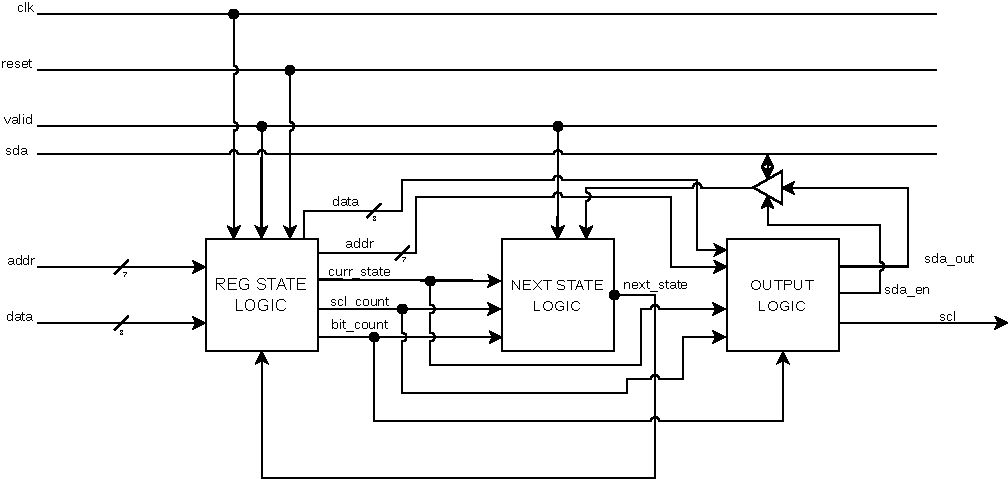
\includegraphics[width=1.0\textwidth]{../imgs/block_diagram.pdf}
    
    \caption{Writing Master block diagram}
    \label{fig:block_diagram}
\end{figure}

The \texttt{REG\_STATE LOGIC} is the synchronous block of the architecture. It manages the registers and handles the reset phase (\texttt{reset} signal is 0). The \texttt{next\_state} signal, coming from the \texttt{NEXT\_STATE LOGIC}, drives the current state register, while the \texttt{addr} and \texttt{data} signals are sampled only when \texttt{valid} is 1. Regarding the counters, the \texttt{scl\_count} signal is incremented by one at every clock cycle, whereas the \texttt{bit\_count} signal increments every 32 clock cycles and only during transmission states. The \texttt{NEXT\_STATE LOGIC} is one of the two combinatorial components and implements the logic to decide the next state where the system will be at the next rising edge of the clock. It needs all the counters to know when the last bit is transmitted and the \IIC{} cycle clock is over. Additionally, it uses the \texttt{valid} signal to start a transaction (consecutive or not) and checks \texttt{sda} signal to know if the acknowledgement signal is received.The last combinatorial component is the \texttt{OUTPUT LOGIC}, which sets the output signals to communicate using the \IIC{} protocol. Based on the \texttt{scl\_count} signal, it generates a clock 32 times slower than the system clock, while the \texttt{bit\_count} signal is used to select the correct bit to transmit.

\newpage